\documentclass{standalone}
\usepackage{tikz}

\begin{document}
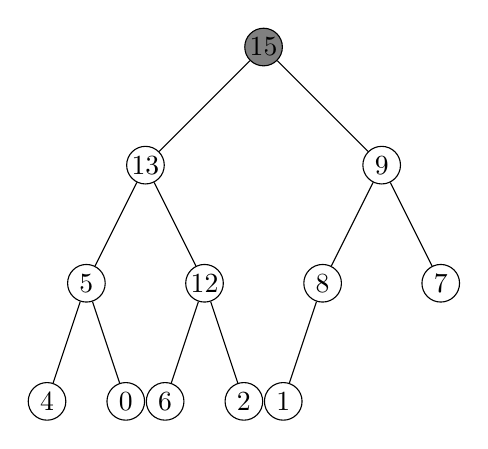
\begin{tikzpicture}[level/.style={sibling distance=30mm/#1},
treenode/.style={align=center, inner sep=0pt, text width=1.2em, text centered},
current/.style={fill=gray}]
    \node [circle,draw,treenode,current] {15}
      child {
        node [circle,draw,treenode] {13}
        child {
            node [circle,draw,treenode] {5}
            child {
                node [circle,draw,treenode] {4}
            }
            child {
                node [circle,draw,treenode] {0}
            }}
        child {
            node [circle,draw,treenode] {12}
            child {
                node [circle,draw,treenode] {6}
            }
            child {
                node [circle,draw,treenode] {2}
            }
        }
      }
      child {
        node [circle,draw,treenode] {9}
        child {
            node [circle,draw,treenode] {8}
            child {
                node [circle,draw,treenode] {1}
            }
            child [missing] {}
        }
        child {
            node [circle,draw,treenode]  {7}
        }
    };
    \end{tikzpicture}
\end{document}